\documentclass[a4paper]{article}

\usepackage[utf8]{inputenc}
\usepackage[T1]{fontenc}      
\usepackage[english]{babel}
\usepackage{array}
% Layout and figures
\usepackage[top=2.5cm,bottom=2.5cm,right=2.5cm,left=2.5cm]{geometry}
\usepackage{subfigure}
\usepackage{rotating}
\usepackage{caption}
% Units and numbers
\usepackage[squaren, Gray]{SIunits}
\usepackage{sistyle}
\usepackage[autolanguage]{numprint}
% Math
\usepackage{amsmath}
\usepackage{amssymb}
\usepackage{amsthm}

% Sets
\newcommand{\Z}{\mathbb{Z}}
\newcommand{\R}{\mathbb{R}}
\newcommand{\C}{\mathbb{C}}
% Links
\usepackage{url}
\usepackage{hyperref}
\hypersetup{
    colorlinks,
    citecolor=black,
    filecolor=black,
    linkcolor=black,
    urlcolor=black
}
\usepackage{tikz}
\usetikzlibrary{arrows,automata}

\definecolor{mygreen}{rgb}{0,0.6,0}
\definecolor{mygray}{rgb}{0.5,0.5,0.5}
\definecolor{mymauve}{rgb}{0.58,0,0.82}

\usepackage{enumerate}
\usepackage{listings}
\lstset{ %
  backgroundcolor=\color{white},   % choose the background color; you must add \usepackage{color} or \usepackage{xcolor}
  basicstyle=\footnotesize,        % the size of the fonts that are used for the code
  breakatwhitespace=false,         % sets if automatic breaks should only happen at whitespace
  breaklines=true,                 % sets automatic line breaking
  captionpos=b,                    % sets the caption-position to bottom
  commentstyle=\color{mygreen},    % comment style
  deletekeywords={...},            % if you want to delete keywords from the given language
  escapeinside={\%*}{*)},          % if you want to add LaTeX within your code
  extendedchars=true,              % lets you use non-ASCII characters; for 8-bits encodings only, does not work with UTF-8
  frame=single,	                   % adds a frame around the code
  keepspaces=true,                 % keeps spaces in text, useful for keeping indentation of code (possibly needs columns=flexible)
  keywordstyle=\color{blue},       % keyword style
  otherkeywords={*,...},           % if you want to add more keywords to the set
  numbers=left,                    % where to put the line-numbers; possible values are (none, left, right)
  numbersep=5pt,                   % how far the line-numbers are from the code
  numberstyle=\tiny\color{mygray}, % the style that is used for the line-numbers
  rulecolor=\color{black},         % if not set, the frame-color may be changed on line-breaks within not-black text (e.g. comments (green here))
  showspaces=false,                % show spaces everywhere adding particular underscores; it overrides 'showstringspaces'
  showstringspaces=false,          % underline spaces within strings only
  showtabs=false,                  % show tabs within strings adding particular underscores
  stepnumber=2,                    % the step between two line-numbers. If it's 1, each line will be numbered
  stringstyle=\color{mymauve},     % string literal style
  tabsize=2,	                   % sets default tabsize to 2 spaces
  title=\lstname                   % show the filename of files included with \lstinputlisting; also try caption instead of title
}

%\usepackage{titlesec}
% New commands
\newcommand{\matlab}{\textsc{Matlab}}
\newcommand{\annexe}{\part{Annexes}\appendix}
\newcommand{\biblioreport}[1]{\bibliographystyle{plain}\bibliography{#1}\nocite{*}}
\DeclareMathOperator{\newdiff}{d} % use \dif instead
\newcommand{\dif}{\newdiff\!}
\newcommand{\fpart}[2]{\frac{\partial #1}{\partial #2}}
\newcommand{\ffpart}[2]{\frac{\partial^2 #1}{\partial #2^2}}
\newcommand{\fdpart}[3]{\frac{\partial^2 #1}{\partial #2\partial #3}}
\newcommand{\fdif}[2]{\frac{\dif #1}{\dif #2}}
\newcommand{\ffdif}[2]{\frac{\dif^2 #1}{\dif #2^2}}
\newcommand{\specialcell}[2][c]{%
\begin{tabular}[#1]{@{}c@{}}#2\end{tabular}}

%\titleformat{\section}
%{\bf\fontsize{20.74}{20.74}\selectfont}
%{\bf\fontsize{20.74}{20.74}\selectfont \thesection \hspace{1 cm}}
%{0 pt}{}{}
%\titlespacing{\section}{10 pt}{10 pt}{20 pt}[10 pt]

\begin{document}
\begin{titlepage}
\newcommand{\HRule}{\rule{\linewidth}{0.5mm}} 
\center 
\textsc{\Large Universit\'e Catholique de Louvain}\\[1cm] 
\textsc{\LARGE LFSAB1105 - Probability and Statistics}\\[0.5cm] 

\HRule \\[0.4cm]
{ \huge \bfseries APP}\\ [0.4cm]
\HRule \\[0.1cm]
\vspace{1cm}
%LOGO UCL
\begin{figure}[ht]
\centering

\includegraphics [height=10cm] {img/ucl}
\end{figure}
\vspace{1cm}
%Author Name
\begin{minipage}{0.7\textwidth}
\begin{center}
\begin{tabular}{lc}
Laurent \textsc{Deleu} & 6040-13-00 \\
Nicolas \textsc{Delinte} & 4801-13-00\\
Damien \textsc{Deprez} & 2893-13-00 \\
Bastien \textsc{Gillon} & 0000-00-00\\

\end{tabular}
\end{center}

\end{minipage}\\[1cm]

%----------------------------------------------------------------------------------------
%	DATE SECTION
%----------------------------------------------------------------------------------------

{\large Ann\'ee acad\'emique 2016-2017}\\[0,25cm] 
{\large \'Ecole Polytechnique de Louvain}\\[1cm]

%----------------------------------------------------------------------------------------
%	LOGO SECTION
%----------------------------------------------------------------------------------------

\begin{center}
  
\includegraphics[width = 20mm]{img/epl.jpg} \hfill
\end{center}
%----------------------------------------------------------------------------------------

\vfill % Fill the rest of the page with whitespace
\end{titlepage}

\tableofcontents

\section{Descriptive statistics}

\begin{enumerate}[(a)]

\item In order to find $t_{p}$ the quantile of order p such that $ P(T \leq t_{p}) = p $, we need to find the solution to the following equation.

$$F_{\alpha , \beta}(t) = \int_{0}^{t_{p}} f_{\alpha , \beta}(t') dt' = p $$
\\
Before integrating the density function, note that :

$$ \frac{\mathrm{d} }{\mathrm{d} x} (1-t^\alpha)^\beta = - \alpha \beta t^{\alpha-1} (1-t^\alpha)^{\beta -1}$$
\\
Thus,

$$F_{\alpha , \beta} (t_p) \quad = \int_{0}^{t_{p}} \alpha \beta t'^{\alpha-1} (1-t'^\alpha)^{\beta -1} dt' = \left [  -(1-t'^\alpha)^\beta \right ]^{t_{p}}_{0} = 1-(1-t_{p}^{\alpha})^\beta$$
\\
The result can be then easily found : $\quad t_p = (1-(1-p)^{\frac{1}{\beta}})^{\frac{1}{\alpha}}$

\item Let's apply the general expression of the moment of order k to our r.v.

\nonumber
\begin{equation} \label{eq1}
\begin{split}
\mathbb{E}(T^k) & = \int_{0}^{1} t^k \alpha \beta t^{\alpha -1} (1-t^\alpha)^{\beta-1} dt \\
 & = \beta \int_{0}^{1} \tau^{\frac{k}{\alpha}} (1-\tau)^{\beta -1} d\tau \\
 & = \beta \frac{\Gamma(\frac{k}{\alpha}+1)\Gamma(\beta)}{\Gamma(\frac{k}{\alpha}+1+\beta)}
\end{split}
\end{equation}
\\
In order to obtain an expression similar to the hint given in the instructions, it necessary to use a variable change : $\tau = t^\alpha$.

\item The previous results allow us to find some statistics describing our variable T.
\\
$\textbf{Mean :} \quad \mu = \mathbb{E}(T) = \beta \frac{\Gamma(\frac{1}{\alpha}+1)\Gamma(\beta)}{\Gamma(\frac{1}{\alpha}+1+\beta)} $
\\
$\textbf{Variance :} \quad \sigma^2 = \mathbb{E}(T^2)-(\mathbb{E}(T))^2 = \beta\frac{\Gamma(\frac{2}{\alpha}+1)\Gamma(\beta)}{\Gamma(\frac{2}{\alpha}+1+\beta)} - \beta^2 \frac{\Gamma(\frac{1}{\alpha}+1)^2\Gamma(\beta)^2}{\Gamma(\frac{1}{\alpha}+1+\beta)^2}$
\\
$\textbf{Median :} \quad t_{0.5} = (1-\frac{1}{2^{\frac{1}{\beta}}})^\frac{1}{\alpha}$
\\
$\textbf{Range :} \quad \textup{Range} = 1$ since $f$ is strictly positive $\forall t \in \left ]  0;1 \right [ $
\\
$\textbf{Interquartile range :} \quad \textup{IQR} = t_{0.75} - t_{0.25} = (1-\frac{1}{4^\frac{1}{\beta}})^\frac{1}{\alpha} - (1-(\frac{3}{4})^\frac{1}{\beta})^\frac{1}{\alpha}$
\\
$\textbf{Coefficient of variation :} \quad cv = \frac{\sigma}{\mu} = \frac{\sqrt{\beta\frac{\Gamma(\frac{2}{\alpha}+1)\Gamma(\beta)}{\Gamma(\frac{2}{\alpha}+1+\beta)} - \beta^2 \frac{\Gamma(\frac{1}{\alpha}+1)^2\Gamma(\beta)^2}{\Gamma(\frac{1}{\alpha}+1+\beta)^2}}}{\beta \frac{\Gamma(\frac{1}{\alpha}+1)\Gamma(\beta)}{\Gamma(\frac{1}{\alpha}+1+\beta)}}$

\item Let's fix our parameters to have an idea of the values of our statistics. For $\alpha_0 = 2$ and $\beta_0 = 4$, we obtain : $\mu = 0.4063$ , $\sigma^2 = 0.0349$ , $t_{0.5} = 0.3989$ , $\textup{IQR} = 0.2778$ and $cv = 0.4596$.

\item The probability that no more than halve of our 50 observations will have a value less than 0.5, can be found in two steps. We firstly calculate the probability that an observation is less than 0.5:

$$P(T<0.5) = \int_{-\infty}^{0.5} = F(0.5) - F(0) = 0.6836 $$
\\
Let's define Y, the total number of successful observations. This new r.v. follows a binomial distribution with $p=0.6836$, our probability of success and $n=50$, our number of trials. Our second step is then to calculate the probability that Y cannot exceed 25.

$$P(X \leq 25) = 1-\sum_{k=25}^{50} C_{k}^{50}p^{k}(1-p)^{50-k} = 0.0022$$

To obtain such a result, it is necessary to make a long summation which can be avoided if we use the Central Limit Theorem. This method uses the fact that the r.v. $\frac{Y-\mu}{\sigma / \sqrt{n}}$ follows a standard normal distribution:

$$P(Y \leq 25) = P\left ( \frac{Y-np}{\sqrt{np(1-p)}} \leq \frac{25-50\cdot0.6836}{\sqrt{50\cdot0.6836\cdot(1-0.6836)}} \right ) \approx P(Z < -2.7915) = 0.0026$$

Our approximated result is not as close as we could have expected, but it is still in the same order of magnitude. This is caused by the huge gap between 25 and 34.2, the mean of our binomial distribution, which depends on our choice of parameters. The further we get away from this mean, the less accurate will be the approximation.

\item From one generated $idd$ sample of size $n = 20$, we observed the following statistics : $\mu = 0.3919$, $\sigma^2 = 0.0432$, $t_0.5 = 0.3922$, $\textup{IQR} = 0.3851$ and $cv = 0.5302$.
These values are very close to the ones calculated previously.

\item As we progressively increase the sample size, the observed statistics approach their theoretical value. We may therefore conclude that the approximation U $\sim$ Unif[0, 1] tends to converge for an increasing size of the sample.

\begin{figure}
    \centering
  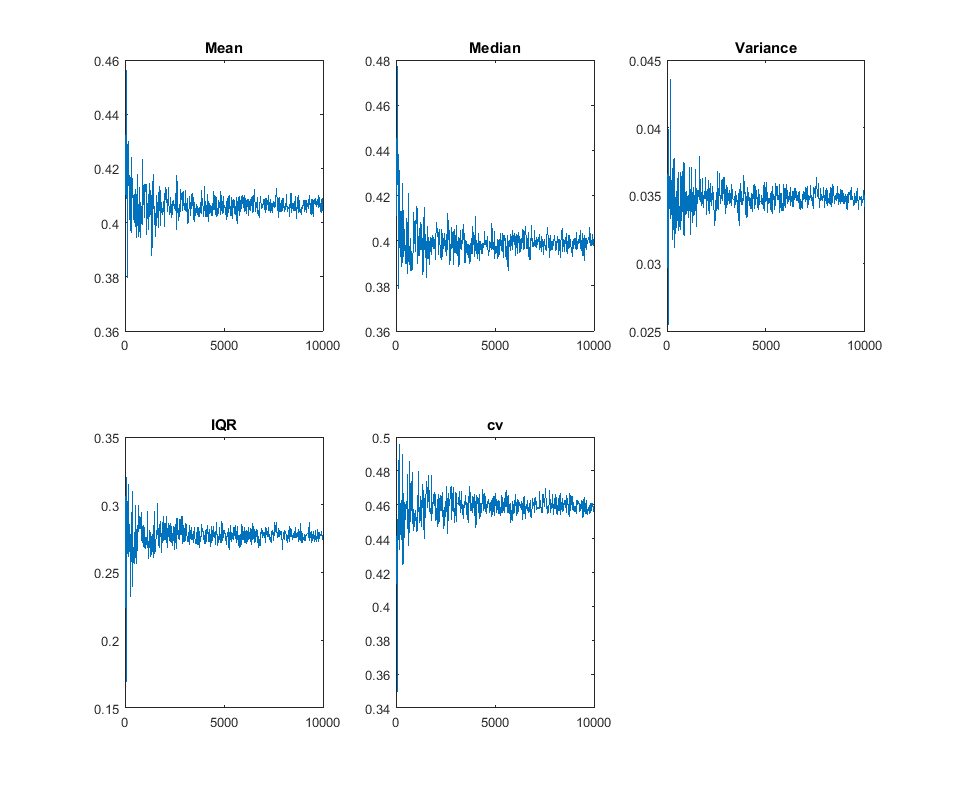
\includegraphics[width = 10cm]{values.png}
  \caption{Convergence of statistics for an increasing sample size}
\end{figure}

\end{enumerate}

\section{Estimation}

\begin{enumerate}[(a)]

\item A first estimator could be taking the rounded value at $ 95\% $ of the ordered sample:
$$\hat{q}_s = T_{[0.95\cdot n]}$$
This estimator would be unbiased if our sample values were following a uniform distribution which is not our case. However, as the median is often approximated by the middle of a sample, we use here the same kind of hypothesis.

\item Seeking a pair of estimators with the method of moments involves finding two equations where our sample moment and the distribution one are equated for both orders. From the expression we need to verify, we see that it is easier to use the moments of order $\alpha$ and $2\alpha$.

$$\mu_\alpha = \mathbb{E}(T^\alpha) = m_\alpha = \frac{1}{n}\sum Y_{i}^{\alpha}$$
$$\mu_{2\alpha} = \mathbb{E}(T^{2\alpha})= m_{2\alpha} = \frac{1}{n}\sum Y_{i}^{2\alpha}$$

Since we know the expression of a moment of order k (found in Part 1), we can develop $\mu_\alpha$ and $\mu_{2\alpha}$. The expression is then simplified using the property $\Gamma(n+1) = n!$

$$\frac{1}{n}\sum T_i^\alpha = \beta \frac{\Gamma(\frac{\alpha}{\alpha}+1)\Gamma(\beta)}{\Gamma(\frac{\alpha}{\alpha}+1+\beta)} = \frac{\beta(\beta-1)!}{(\beta+1)!} = \frac{1}{\beta+1}$$

$$\frac{1}{n}\sum T_i^{2\alpha} = \frac{\Gamma(\frac{2\alpha}{\alpha}+1)\Gamma(\beta)}{\Gamma(\frac{2\alpha}{\alpha}+1+\beta)} = \frac{2\beta(\beta-1)!}{(\beta+2)!} = \frac{2}{(\beta+2)(\beta+1)}$$

By rearranging the terms of our first line, we find an expression for $\hat{\beta}_M$ which is the second equation we were looking for. By injecting this into our second line, we then obtain the first equation to be verified after another rearrangement of terms.

$$\hat{\beta}_M = \frac{n}{\frac{1}{n}\sum T_i^{\hat{\alpha}_M}} - 1$$

$$\left ( \frac{1}{n}\sum T_i^{2\hat{\alpha}_M} \right )  \left (n + \frac{1}{n}\sum T_i^{\hat{\alpha}_M} \right )  \left ( \frac{1}{n}\sum T_i^{\hat{\alpha}_M} \right )^{-2} = 2$$

\item We seek the two parameters $\hat{\alpha}_L$ and $\hat{\beta}_L$ that maximise our likelihood function. 

$$L(T_i|\alpha,\beta) = \prod_{i=1}^{n} f_{\alpha,\beta}(T_i) = \prod_{i=1}^{n} \alpha\beta T_i^{\alpha-1}(1-T_i^\alpha)^{\beta-1}$$

In order to make the following derivations easier, we apply the natural logarithm to our function. This will not change the solution of our maximisation problem as the logarithm is a monotonically increasing function.

$$l(T_i|\alpha,\beta) = \ln(L(T_i|\alpha,\beta)) = \sum_{i=1}^n \left [ \alpha\beta T_i^{\alpha-1}(1-T_i^\alpha)^{\beta-1} \right ]$$

We now derive our function with respect to each of our parameters and find the zeros of these derivatives.

$$ \frac{\partial l(\alpha, \beta)}{\partial \alpha} = \frac{n}{\alpha} + \sum_{i=1}^n \ln(T_i) + (1-\beta) \sum_{i=1}^{n} \frac{\ln(T_i) T_i^\alpha}{1-T_i^\alpha} = 0$$
$$ \frac{\partial l(\alpha, \beta)}{\partial \beta} = \frac{n}{\beta} + \sum_{i=1}^{n} \ln(1- T_i^\alpha)=0$$

As for the previous method, we isolate $\hat{\beta}_L$ in the second line and then inject its expression in the first one. After a rearrangement of terms, we obtain the sought expressions.

$$\frac{1}{\hat{\alpha}_L} + \left ( \frac{1}{\sum_{i=1}^n \ln(1-T_i^{\hat{\alpha}_L})} + \frac{1}{n}\right ) \sum_{i=1}^{n}\frac{\ln(T_i)T_i^{\hat{\alpha}_L}}{1-T_i^{\hat{\alpha}_L}} = - \frac{1}{n} \sum_{i=1}^n \ln(T_i)$$

$$\hat{\beta}_L = \frac{-n}{\sum_{i=1}^n \ln(1-T_i^{\hat{\alpha}_L})}$$

\item We know that our sample follows a $f_{\alpha,\beta}$ distribution and we now have estimators for the parameters $\alpha$ and $\beta$. We can therefore use our relation from Part 1 between a quantile of order p and the distribution parameters to have the expression of a new estimator for $t_{0.95}$.

$$ \hat{q}_M = (1-0.05^{\frac{1}{\hat{\beta}_M}})^{\frac{1}{\hat{\alpha}_M}}$$

$$ \hat{q}_L = (1-0.05^{\frac{1}{\hat{\beta}_L}})^{\frac{1}{\hat{\alpha}_L}}$$

\end{enumerate}

\section{Simulations}

\section{Linear regression and ANOVA}

\appendix

\section{MatLab Code}
\end{document}
